\begin{figure*}
  \centering

\begin{minipage}{\textwidth}
\begin{subfigure}[b]{0.4\textwidth}
\centering
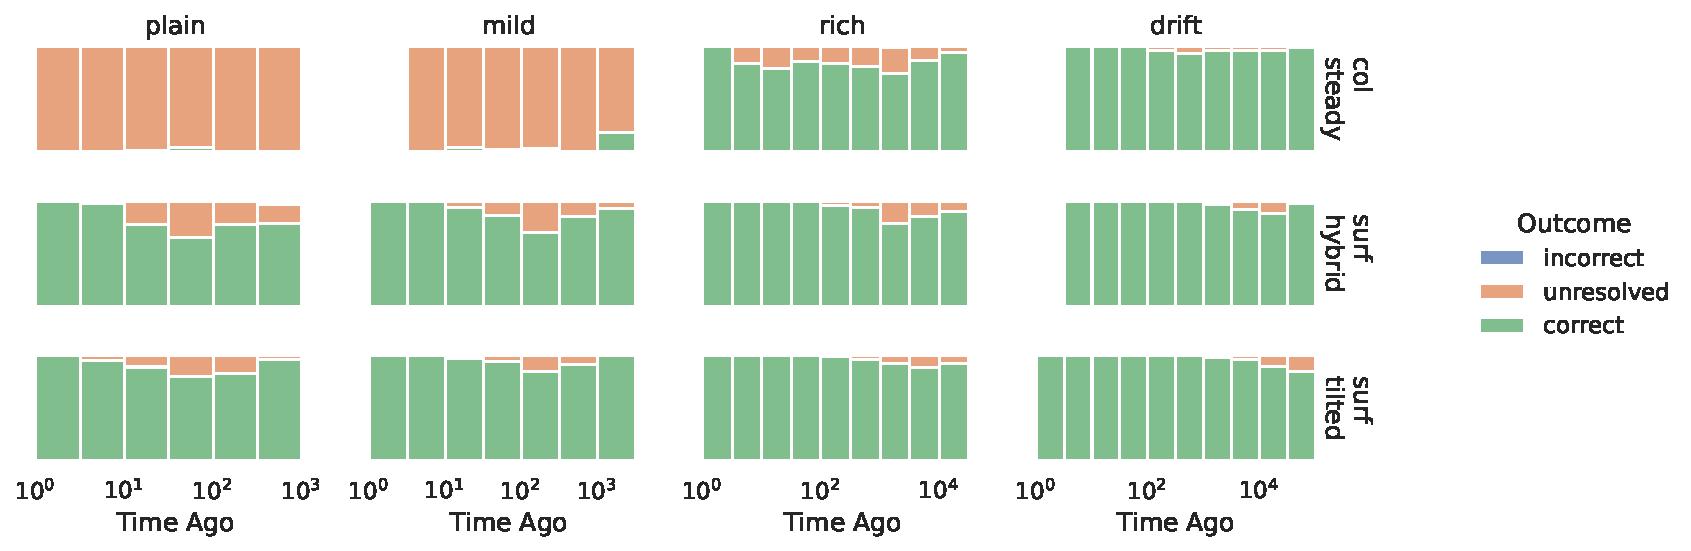
\includegraphics[height=1.2in,trim={0 0 5cm 0},clip]{binder/binder/teeplots/annotation-size=256+col=scenario+differentia-width=8+hue=outcome+kind=hist+multiple=fill+row=algo+scale=npop65536-ngen100000+viz=displot+x=time-ago+ext=}
\footnotesize
\caption{byte differentia outcomes; 256-bit annotation}
  \label{fig:bit-vs-byte-summary-byte-outcomes}
  \end{subfigure}%
\begin{subfigure}[b]{0.6\textwidth}
\centering
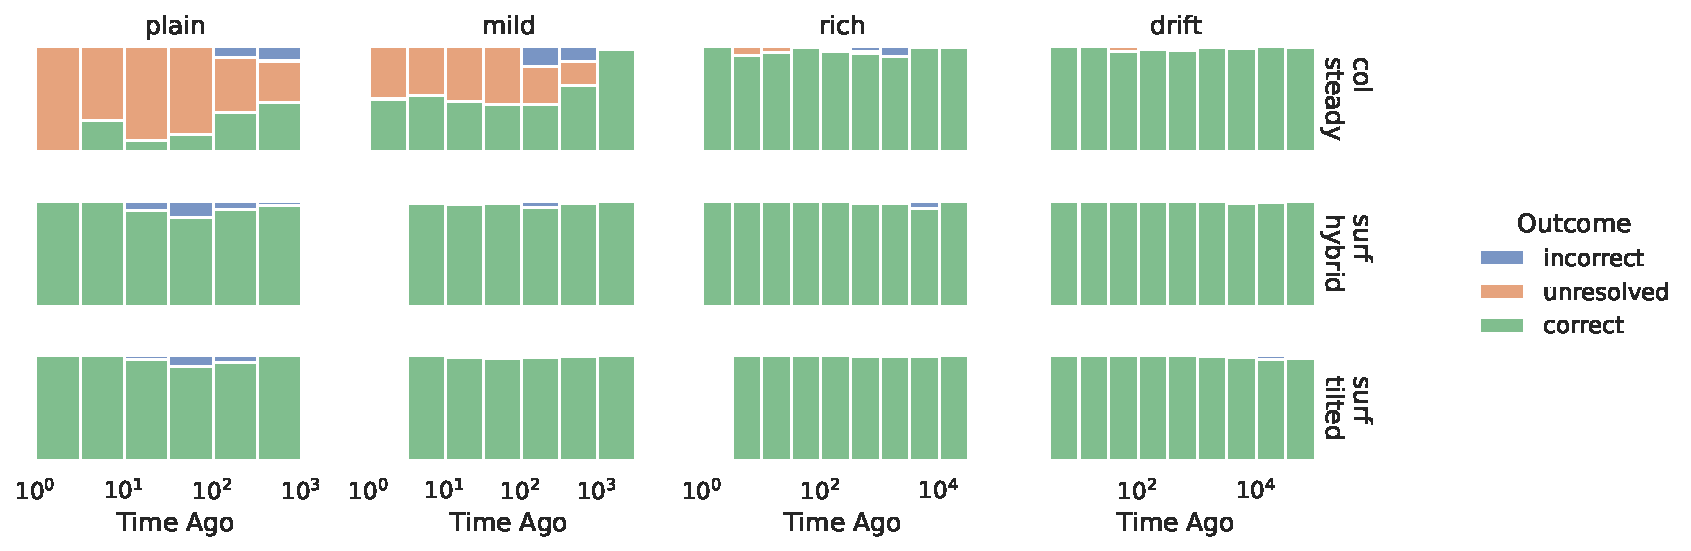
\includegraphics[height=1.2in]{binder/binder/teeplots/annotation-size=256+col=scenario+differentia-width=1+hue=outcome+kind=hist+multiple=fill+row=algo+scale=npop65536-ngen100000+viz=displot+x=time-ago+ext=}
\footnotesize
\caption{bit differentia outcomes; 256-bit annotation}
\label{fig:bit-vs-byte-summary-bit-outcomes}
\end{subfigure}
% \begin{subfigure}[b]{0.6\textwidth}
% \centering
% 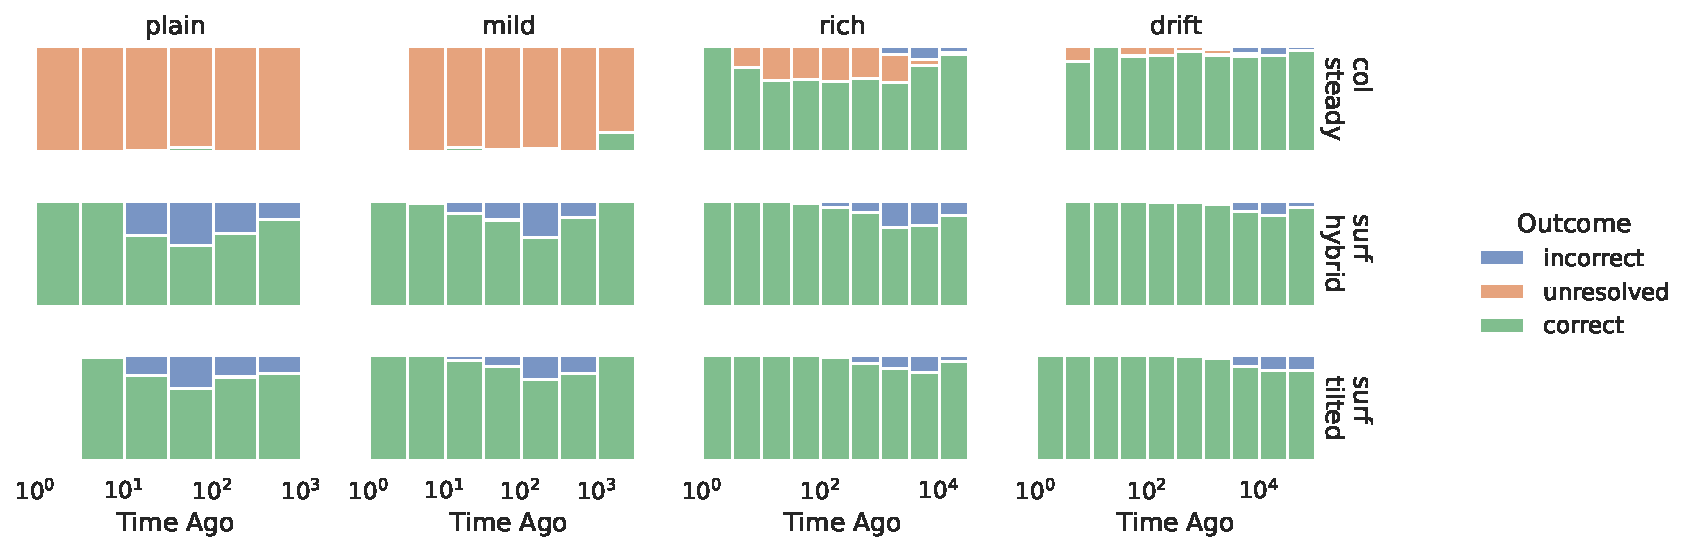
\includegraphics[height=1.2in]{binder/binder/teeplots/annotation-size=32+col=scenario+differentia-width=1+hue=outcome+kind=hist+multiple=fill+row=algo+scale=npop65536-ngen100000+viz=displot+x=time-ago+ext=}
% \caption{32-bit annotation, bit differentia}
% \end{subfigure}
\end{minipage}
% \begin{subfigure}[b]{0.4\textwidth}
%   \centering
%   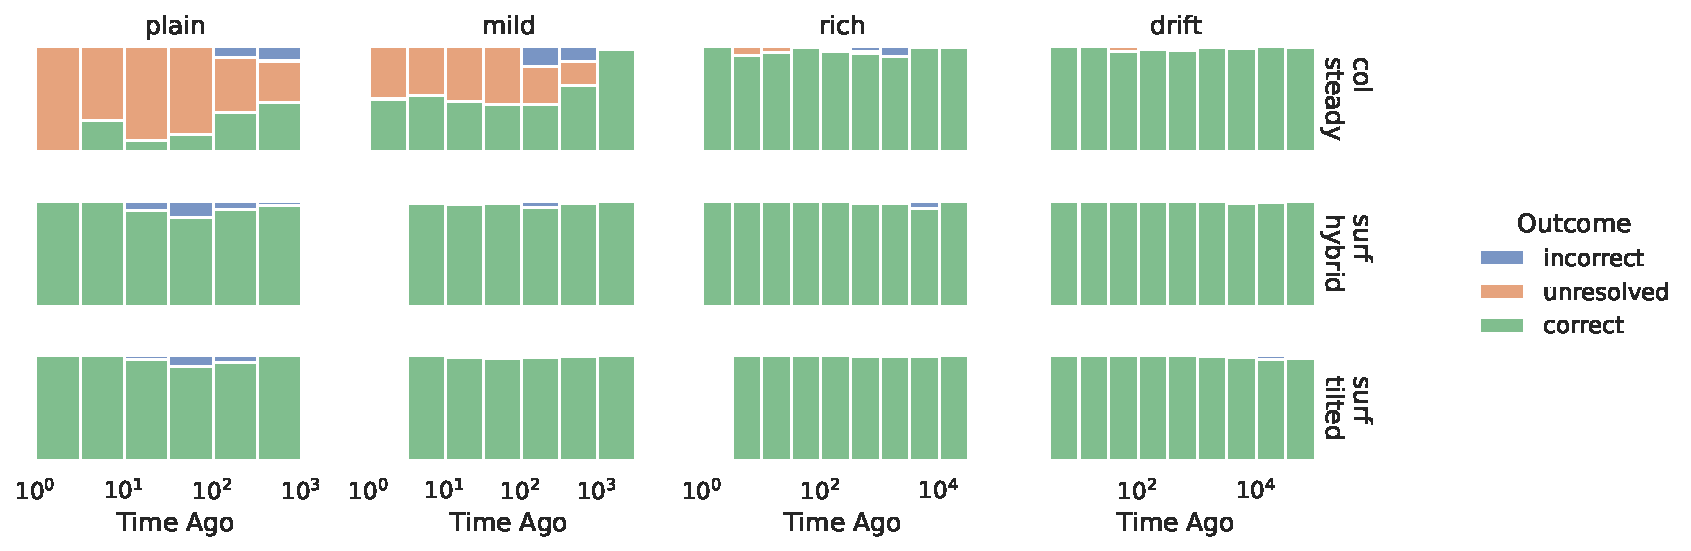
\includegraphics[height=1.2in,trim={0 0 5cm 0},clip]{binder/binder/teeplots/annotation-size=256+col=scenario+differentia-width=1+hue=outcome+kind=hist+multiple=fill+row=algo+scale=npop65536-ngen100000+viz=displot+x=time-ago+ext=}
%   \caption{reconstruction outcomes; 256-bit annotation, bit differentia}
%   \end{subfigure}%
  \begin{subfigure}[b]{\textwidth}
    \centering
    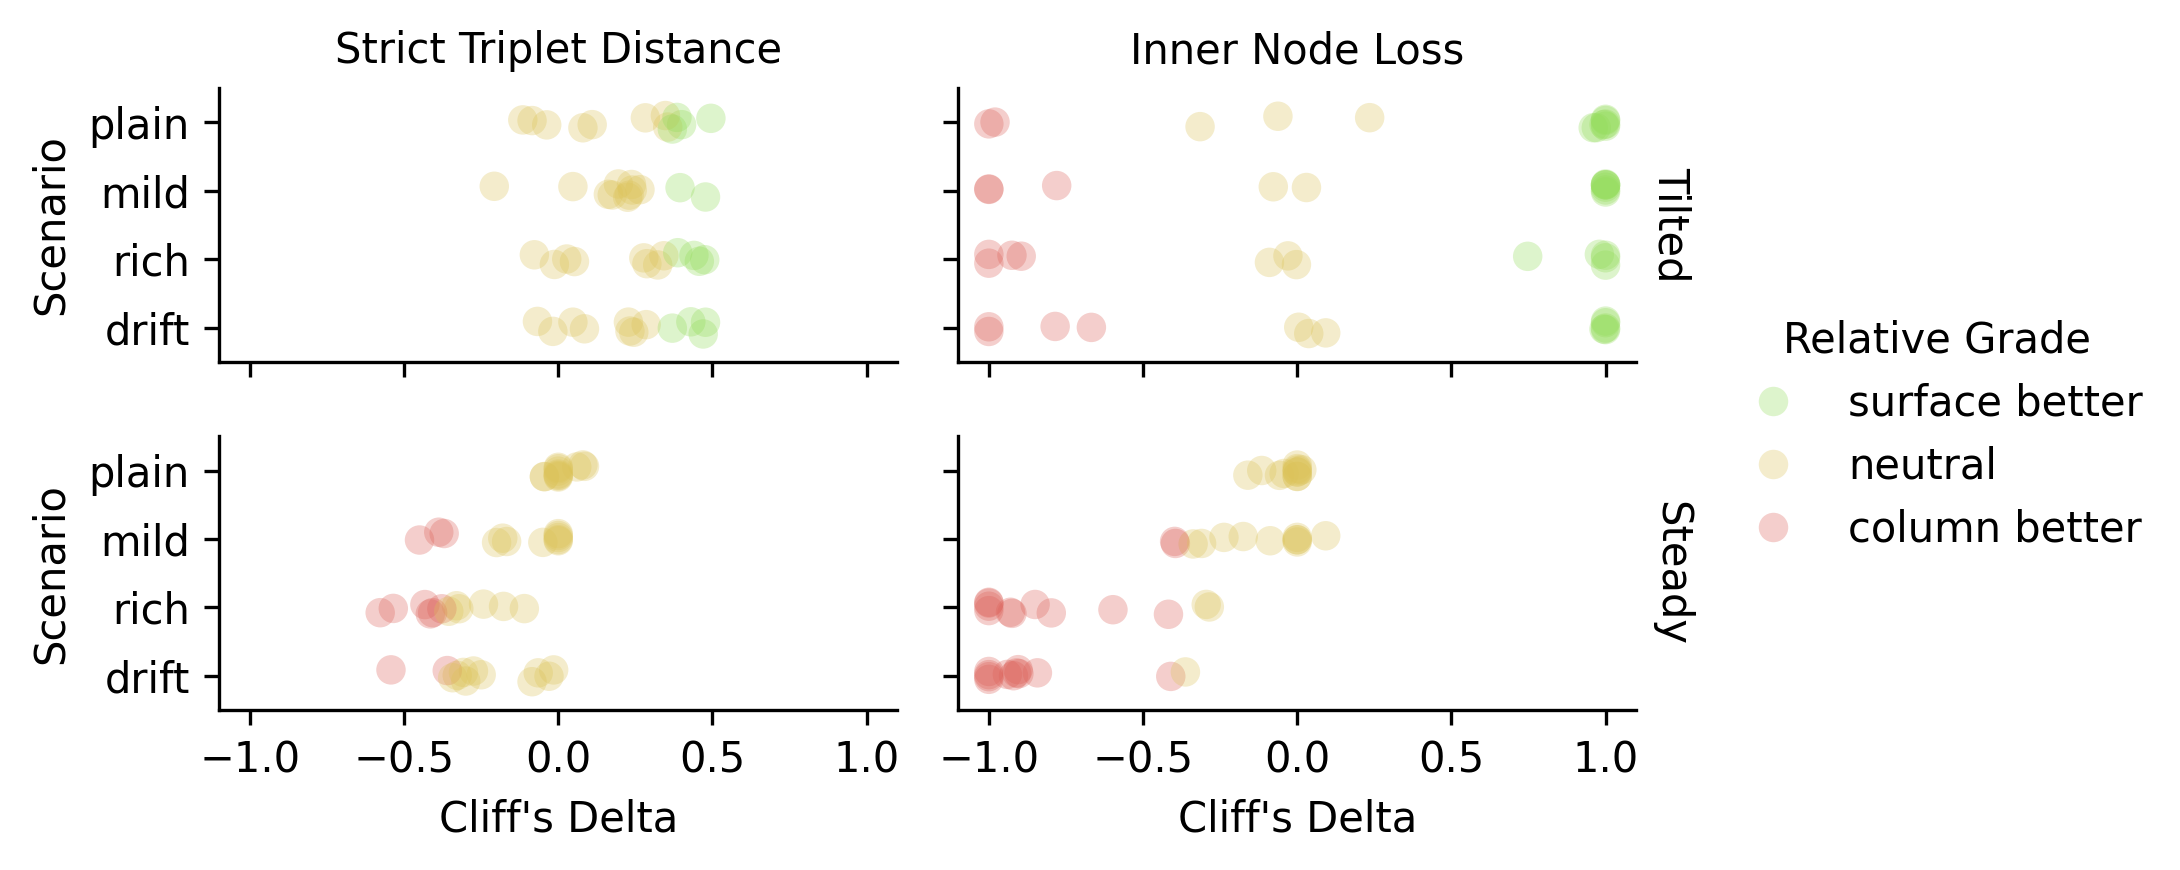
\includegraphics[width=0.8\linewidth]{binder/binder/bit-vs-byte/teeplots/col=metric+hue=relative-grade+kind=strip+row=policy+viz=catplot+x=cliff-s-delta+y=scenario+ext=}
    \footnotesize
    \caption{Reconstruction quality of byte differentia, relative to bit differentia; 256-bit size annotation}
  \label{fig:bit-vs-byte-summary-quality}
  \end{subfigure}%
\caption{%
  \textbf{How does differentia width affect reconstruction quality?}
  \footnotesize
   Top panels show reconstruction outcomes for phylogenetic branching events (Figure \ref{fig:hstrat-failure-modes}) under bit- and byte-width differentiae, respectively.
   Outcomes are binned by time ago (ranging from most recent to most ancient).
   Bottom panel compares reconstruction quality metrics between reconstructions from annotations with bit- and byte-width differentiae.
   Color coding indicates significance, with red indicating better bit-width differentia performance and green indicating better byte-width differentia performance.
   Byte-width differentiae consistently underperform bit-width differentia in inner node loss and strict triplet distance measures.
   However, byte-width differentiae outperform bit-width differentia in the lax triplet distance measure, which does not penalize polytomy triplets, i.e., isolating incorrect reconstruction from unresolved reconstruction (Figure \ref{fig:hstrat-failure-modes}).
  See Supplementary Figure \ref{fig:bit-vs-byte} for listing of effects by sensitivity analysis condition \citep{moreno2024supplemental}.
}
  \label{fig:bit-vs-byte-summary}

\end{figure*}
